\section{Supporting Materials}
% ==================================================================================================
\subsection{Notation}\label{app.notation}
Table~\ref{tab:notation} summarizes our notation,
and any corresponding parameters from \cite{Arenas2020}.
\begin{table}[ht]
  \centering
  \caption{Notation}
  \begin{tabular}{ccl}
  \toprule
   Symbol   &        Symbol        & Definition                     \\
   in this  & in \cite{Arenas2020} &                                \\
  \midrule
     $g$    &         $i$          & home patch                     \\
    $g'$    &         $j$          & other patch                    \\
    $g^*$   &         ---          & visited patch                  \\
     $a$    &         $g$          & self age group                 \\
    $a'$    &         $h$          & other age group                \\
     $y$    &         ---          & contact type                   \\
     $n$    &         ---          & home FSA                       \\
    $n'$    &         ---          & visited FSA                    \\
     $i$    &         $m$          & infection state                \\
     $P$    &         $N$          & population size                \\
     $B$    &         $R$          & mobility matrix                \\
     ---    &         $M$          & convenience mobility matrix    \\
  $\lambda$ &        $\Pi$         & force of infection             \\
   $\rho$   &         $p$          & mobility factor                \\
     $h$    &         ---          & home pool contact proportion   \\
     $C$    &         $k$          & contacts per person            \\
     $X$    &         ---          & total absolute contacts        \\
  $\theta$  &         $C$          & contacts age distribution      \\
   $\phi$   &         ---          & odds of mobility if unobserved \\
   $\psi$   &         ---          & relative time away from home   \\
  \bottomrule
\end{tabular}
  
  \label{tab:notation}
\end{table}
% ==================================================================================================
\subsection{Interpretation of ``Non-mobile''}\label{app.nonmobile}
As described in \S~\ref{meth.orig}, \citet{Arenas2020} model the degree of mobility of age group $a$
using a parameter $\rho_a$ (our notation),
incorporated into a convenience matrix $M_{gg'}$ per Eq.~(\ref{eq:Arenas.M})\,/\,(\ref{eq:Arenas.M.app}),
repeated here for reference:
\begin{equation}\label{eq:Arenas.M.app}
  M_{gg'a} = (1-\rho_a)\,\delta_{gg'} + \rho_a B_{gg'a}
\end{equation}
The implicit assumption of this approach is that
non-mobile individuals may form contacts with visitors to their patch, which may not be as intended.
The proposed approach to modelling mixing can avoid this assumption if desired.
Figure~\ref{fig:nm} explores the potential influence of this assumption on network connectivity,
as measured by the expected proportion of contacts formed with other patches, in a toy example.
The example with 3 patches, each having equal population size and random mobility ($B_{gg'} = 1/N_{g'}$).
Age is not considered.
\par
By simulating mixing between non-mobile individuals and mobile visitors
(Figures~\ref{fig:nm.half.stay}~\&~\ref{fig:nm.diff.stay})
the proportions of contact made with other patches increases for all patches,
as compared to the proposed approach
(Figures~\ref{fig:nm.half.home}~\&~\ref{fig:nm.diff.home}).
The difference is largest in the context of differential mobility by patch
(Figures~\ref{fig:nm.diff.stay}~vs~\ref{fig:nm.diff.home}).
\begin{figure}[ht]
  \newcommand{\threepct}[3]{#1,~#2,~#3\,\%}
  \centering
  \begin{subfigure}{0.49\linewidth}
    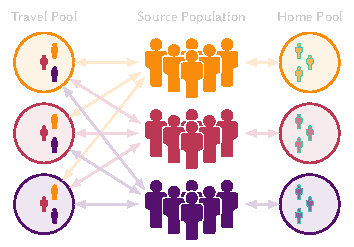
\includegraphics[width=\linewidth]{pools-half-home}
    \caption{Non-mobile = stay at home, all patches 50\% mobile}
    \label{fig:nm.half.home}
    \floatfoot{Contacts formed with other patches:\\
      33\% if non-mobile have equal contact rates vs mobile\\
      44\% if non-mobile have 1/2 contact rates vs mobile}
  \end{subfigure}\hfill%
  \begin{subfigure}{0.49\linewidth}
    \centering
    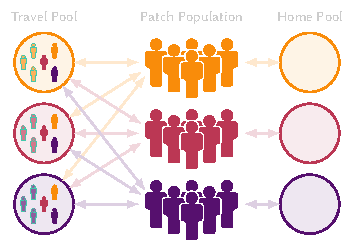
\includegraphics[width=\linewidth]{pools-half-stay}
    \caption{Non-mobile = stay in patch, all patches 50\% mobile}
    \label{fig:nm.half.stay}
    \floatfoot{Contacts formed with other patches:\\
      50\% if non-mobile have equal contact rates vs mobile\\
      59\% if non-mobile have 1/2 contact rates vs mobile}
  \end{subfigure}\medskip\par
  \begin{subfigure}{0.49\linewidth}
    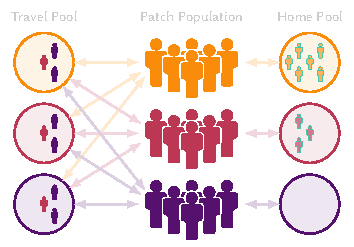
\includegraphics[width=\linewidth]{pools-diff-home}
    \caption{Non-mobile = stay at home, patches \threepct{0}{50}{100} mobile}
    \label{fig:nm.diff.home}
    \floatfoot{Contacts formed with other patches:\\
      \threepct{0}{33}{33} if non-mobile have equal contact rates vs mobile\\
      \threepct{0}{44}{33} if non-mobile have 1/2 contact rates vs mobile}
  \end{subfigure}\hfill%
  \begin{subfigure}{0.49\linewidth}
    \centering
    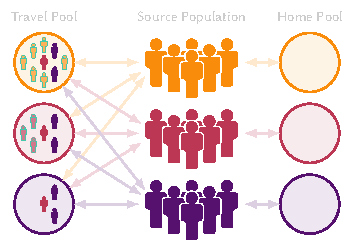
\includegraphics[width=\linewidth]{pools-diff-stay}
    \caption{Non-mobile = stay in patch, patches \threepct{0}{50}{100} mobile}
    \label{fig:nm.diff.stay}
    \floatfoot{Contacts formed with other patches:\\
      \threepct{33}{48}{59} if non-mobile have equal contact rates vs mobile\\
      \threepct{50}{58}{52} if non-mobile have 1/2 contact rates vs mobile}
  \end{subfigure}
  \caption{Mixing implications for two assumptions about the behaviour of non-mobile populations:
    ``stay at home'' (\subref{fig:nm.half.home},\subref{fig:nm.diff.home}):
    no contacts with other patches (proposed here); vs
    ``stay within patch'' (\subref{fig:nm.half.stay},\subref{fig:nm.diff.stay}):
    no travel, but may form contacts with travellers from other patches (as in \cite{Arenas2020}).}
  \floatfoot{
    Non-mobile populations are indicated with faded colour and green outline;
    patch-specific values ordered from top (yellow) to bottom (purple).
    Additional assumptions:
    large population size;
    equal population sizes and contact rates by patch;
    random mobility (equal probability of visiting any patch if mobile).}
  \label{fig:nm}
  % MH: Very cool - critical appendix figure!
\end{figure}
\clearpage
% ==================================================================================================
\subsection{Deriving the Mobility Matrix}\label{app.mob}
Here we describe the methods used to obtain the mobility matrix $B_{gg'}$,
representing the expected proportions of individuals residing in decile/patch $g$,
% MH: instead of "/" would recommend putting patch in brackets: decile (i.e. geographic patch)
who travel to decile/patch $g'$ each day,
based on mobile device data.
% MH: Would recommend adding terminology to indicate this is an applied example
% so individuals from outside of Ontario/Canada don't get confused with decile and FSA terminology.
% Could also highlight "for applied example" in A.3 title.
We will begin by producing the FSA-level mobility matrix $B_{nn'}$.
% --------------------------------------------------------------------------------------------------
\subsubsection{Data}\label{app.mob.data}
The raw data represent logs of: timestamp, geolocation (latitude\,/\,longitude), and unique device ID.
A log entry (``ping'') is generated when an app on the device
requests the current geolocation from the service provider.
Geolocation is logged using Geohash level 6 (1.2 \,km $\times$ 609.4\,m).
The midpoint of each Geohash is then compared to boundary files representing all 513 Ontario FSAs%
\footnote{\hreftt{https://www150.statcan.gc.ca/n1/en/catalogue/92-179-X}}
to determine which FSA the ping is attributed to.
The following definitions were then used to determine device mobility.
\par
The ``home FSA'' of each unique device is defined as
the FSA with the greatest daily-average time between 8:00\,pm--5:00\,am during each calendar month.
Devices for which it was not possible to determine the home FSA were excluded from all further analysis.
\par
The ``visited FSAs'' represent FSAs a device travelled to within a 24-hour period,
as defined by at least 2 consecutive pings spanning at least 2 hours within the FSA.
By this definition, it was possible for a device to visit multiple FSAs, or no FSA during a given day.
Repeated visits to the same FSA by the same device on the same calendar date are treated as a single visit.
\par
The ``time away from home'' represents the proportion of time each device
was estimated to be away from the home dwelling (not just FSA),
as defined by the Geohash 6 tile with the greatest daily-average time between 8:00\,pm and 5:00\,am each month.
% MH: Given you have already defined home FSA above think this is unneccessary.
% Also reads as if the "time away from home" is defined by
% the greatest daily average time between 8:00pm  to 5:00am each month.
\par
These definitions were applied to each calendar month $t$ from Jan 2020--Dec 2020 (12 months) to compute:
the mean number of devices with home FSA $n$ per day, denoted $H_{nt}$ or ``observed devices'';
the mean number of devices with home FSA $n$ that visited FSA $n'$ per day, denoted $V_{nn't}$, or ``device visits''; and
the mean proportion of time each device spent outside the home per day for each FSA, denoted $W_{nt}$.
% --------------------------------------------------------------------------------------------------
\subsubsection{Inter-FSA Mobility}\label{app.mob.inter}
The inter-FSA mobility matrix $B_{nn't}$ ($n \ne n'$) could be defined as
the proportion of observed devices that travelled to each FSA ($V_{nn't} / H_{nt}$).
However, the following analysis of the data suggested that such an approach may bias estimates of mobility.
A reference period $t_0$ was defined as Jan--Feb 2020, to reflect pre-pandemic conditions.
The expected values of $H_{nt}$ and $V_{nt} = \sum_{n' V_{nn't}}$ for each FSA during this period were then
computed and compared to the expected values during each subsequent month.
Figure~\ref{fig:RHVt} plots the distribution of ratios
$H_{nt} / H_{nt_0}$ (\subref{fig:RHt}) and $V_{nt} / V_{nt_0}$ (\subref{fig:RVt})
across all 513 FSAs, for each month.
These ratios illustrate that both $V_{nt}$ and $H_{nt}$ were influenced (reduced) by pandemic restrictions,
and thus $V_{nn't} / H_{nt}$ would overestimate mobility.
The trend in $H_{nt}$ might be because apps accessing geolocation services are only opened
after the user intends to travel, such as map-related apps.
\begin{figure}
  \centering
  \begin{subfigure}{0pt}\refstepcounter{subfigure}\label{fig:RHt}\end{subfigure}%
  \begin{subfigure}{0pt}\refstepcounter{subfigure}\label{fig:RVt}\end{subfigure}%
  \begin{subfigure}{0pt}\refstepcounter{subfigure}\label{fig:RH0Vt}\end{subfigure}%
  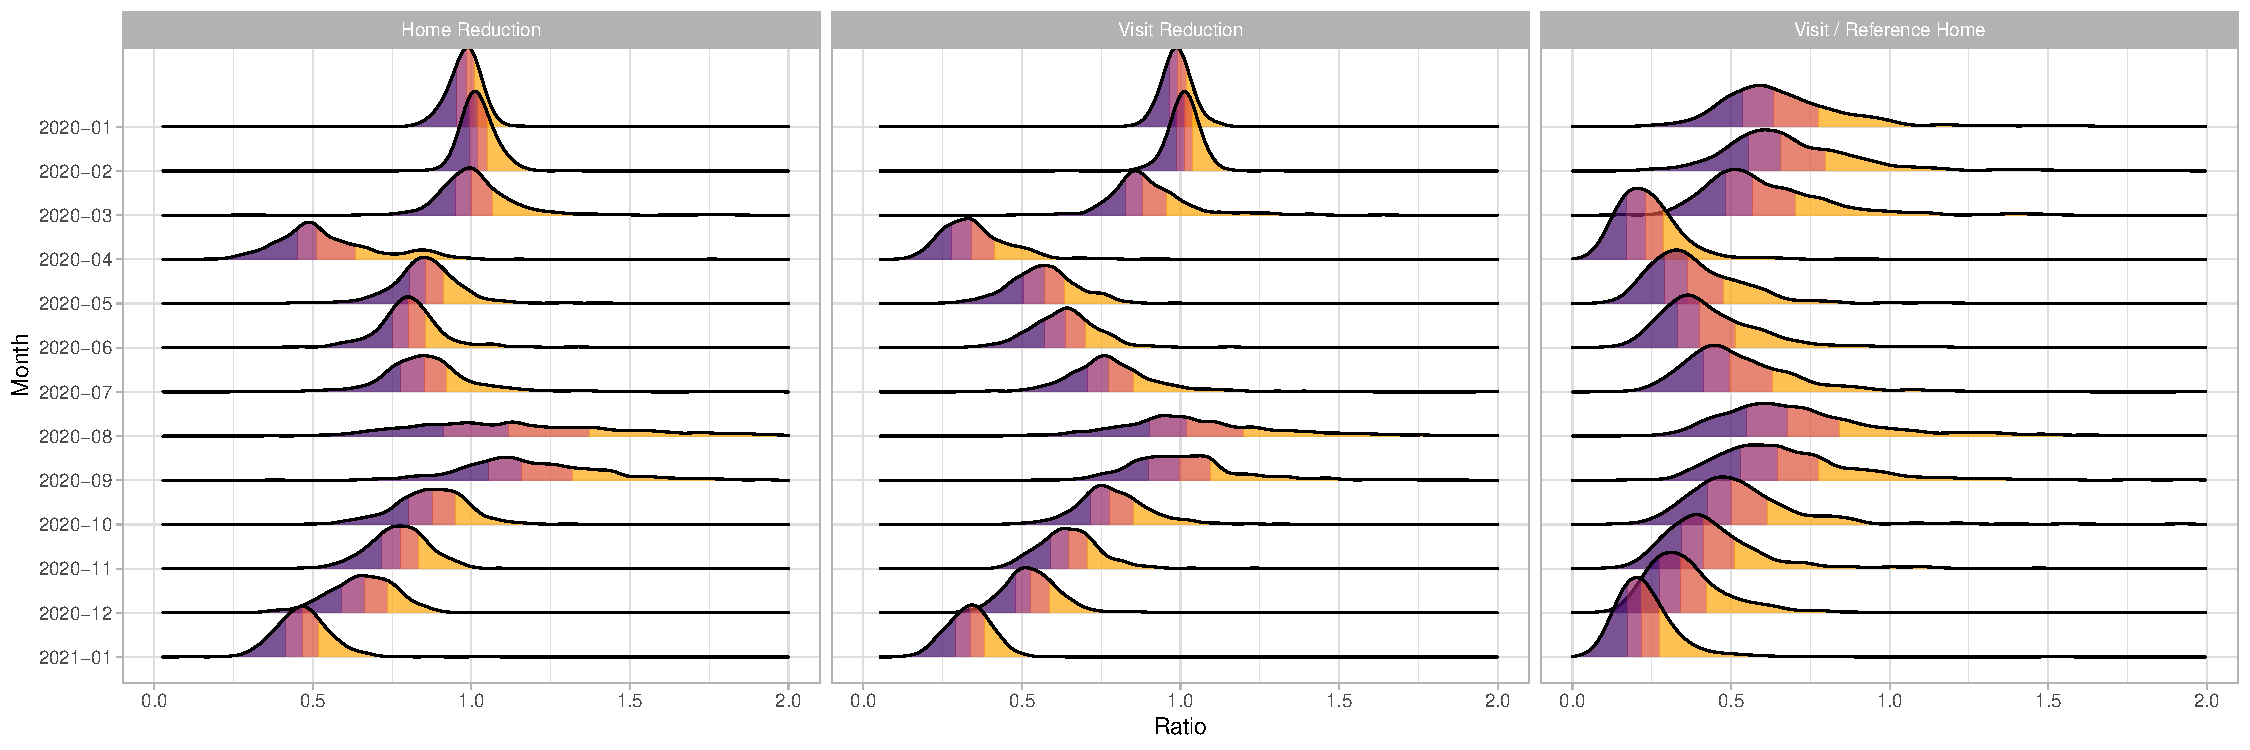
\includegraphics[width=\linewidth]{devices-ratios}
  \caption{Ratios of (\subref{fig:RHt}) observed devices at home
    and (\subref{fig:RVt}) total device visits
    during each month versus during the reference period (Jan--Feb 2020),
    suggesting that the proportion of observed devices travelling each month
    alone is not reflective of true mobility or (\subref{fig:RHt}) would be 1;
    (\subref{fig:RH0Vt}) adjusted mobility measure: ratio of
    device visits each month from versus
    the number of observed devices at home during the reference period}
  \label{fig:RHVt}
  \floatfoot{Distributions show the density of ratio values across all 513 FSAs;
    coloured segments indicate the 4 quantiles of each distributions.}
\end{figure}
\par
To address this bias, we chose $H_{nt_0}$ as a more reliable denominator,
% Inherent in the definition of Hnto
and thus modelled mobility using: $V_{nn't} / H_{nt_0}$ (Figure~\ref{fig:RH0Vt}).%
\footnote{One limitation of this approach is that the reference period only includes winter months,
  which may not be representative of mobility year-round.
  Indeed, all three ratios in Figure~\ref{fig:RHVt} have substantial tails above 1 during Aug--Sept 2020,
  suggesting that mobility was higher during that period versus the pre-pandemic reference period.}
However, the results of Figure~\ref{fig:RHVt} also suggest that
unobserved devices are less mobile than observed devices;
thus the unobserved devices would not have the same expected mobility as the observed devices.
To account for this observation, we first estimated the total number of devices per FSA, denoted $D_n$,
using Statistics Canada data on smart-phone ownership by age group.%
\footnote{\hreftt{https://www150.statcan.gc.ca/t1/tbl1/en/tv.action?pid=2210011501}}
Based on these data, we estimate that $H_{nt}$ represents
2.2~[IQR:~1.9,~2.6]\,\% of devices pre-pandemic, and
1.8~[IQR:~1.4,~2.3]\,\% after from March 2020--Jan 2021.
The number of unobserved devices in FSA $n$ before the pandemic is therefore $D_n - H_{nt_0}$.
\par
During the pandemic, additional devices go unobserved ($H_{nt}$ decreases)
but we assume that the newly unobserved devices do not travel.
Therefore, the number of devices that may travel unobserved
is a proportion of $D_n - H_{nt_0}$, not a proportion of $D_n - H_{nt}$.
Since we have no data on these individuals, we assume that they are mobile
at a rate $\phi_1 < 1$ (default 0.9) relative to the observed devices.
Similarly, for individuals who do not own devices ($P_n - D_n$) we assume that they are mobile
at a rate $\phi_2 < 1$ (default 0.9) relative to the observed devices.
% Think it might be worth providing a rationale for why
% we assume observed devices are more mobile than those who are unobserved and those without devices
% (potentially greater intent to travel if we are observing)
Thus, the total proportion of individuals in FSA $n$ who travel to FSA $n'$ during month $t$ is modelled~as:
\begin{equation}\label{eq:Bnnt.inter}
  B_{nn't \,(n\ne n')} = \frac{V_{nn't}}{H_{n0}} \big[
  \underbrace{1\vphantom{\phi}}_{\textrm{(a)}}
  + \underbrace{\phi_1 \left(D_n - H_{n0}\right)}_{\textrm{(b)}}
  + \underbrace{\phi_2 \left(P_n - D_n\right)}_{\textrm{(c)}} \big] P_n^{-1}
\end{equation}
where (a) represents the observed devices,
(b) represents unobserved devices, and
(c) represents individuals without devices.
% --------------------------------------------------------------------------------------------------
\subsubsection{Intra-FSA Mobility}\label{app.mob.intra}
Since device visits to other FSA $V_{nn't}$ do not include ``visits'' within the home FSA,
the proportion of individuals who are mobile (making contacts) within their home FSA is not yet determined.
During the reference period, we assume that
all individuals who do not travel to other FSAs are still mobile within their home FSA:
\begin{equation}\label{eq:Bnnt.intra.t0}
  B_{nn't_0\,(n = n')} = 1 - \sum_{n'} B_{nn't_0\,(n \ne n')}
\end{equation}
During pandemic months, we assume that
a proportion of such individuals remain mobile within their home FSA;
this proportion is derived from the time away from home $W_{nt}$ as follows.
We assume that individuals who are mobile within their home FSA
spend $\psi \le 1$ (default 1) as much time away from home as
those who are mobile within other FSAs.
Thus, the model for $W_{nt}$ is:
\begin{equation}\label{eq:Wnt}
  W_{nt} = W^*_n \left(\psi B_{nn't\,(n = n')} + \sum_{n'} B_{nn't\,(n \ne n')} \right)
\end{equation}
where $W^*_n$ is the expected proportion of time away from home
among travellers from FSA $n$ to other FSAs.
During the reference period, all individuals are mobile so $B_{nn't_0\,(n = n')}$ is known, and
$W^*_n$ can be calculated by rearranging Eq.~(\ref{eq:Wnt}).
Then, during the pandemic months, the observed $W_{nt}$ can be used to infer $B_{nn't\,(n = n')}$ as:
\begin{equation}\label{eq:Bnnt.intra.t}
  B_{nn't\,(n = n')} = \left(\frac{W_{nt}}{W^*_n} - \sum_{n'} B_{nn't\,(n \ne n')}\right) \psi^{-1}
\end{equation}
Figure~\ref{fig:W} plots the distribution of expected times away from home $W_{nt}$
in hours (\subref{fig:W-hours}) and relative to the reference period $W_{nt_0}$ (\subref{fig:W-relative}).
\par
During the pandemic months, $B_{nn't}$ will sum to less than 1 for many FSAs;
this is desirable, since we interpret $1 - \sum_{n'} B_{nn't}$ as
the expected proportion of individuals in FSA $n$
who did not leave the home each day during month~$t$,
and thus would not form any mobility-related contacts.
Similarly, if $B_{nn't}$ sums to greater than 1, the net result in the force of infection is that
individuals may form more contacts than expected from the reference period,
which is also usually acceptable (such as during Aug--Sept 2020).
\begin{figure}
  \centering
  \begin{subfigure}{0.4\linewidth}
    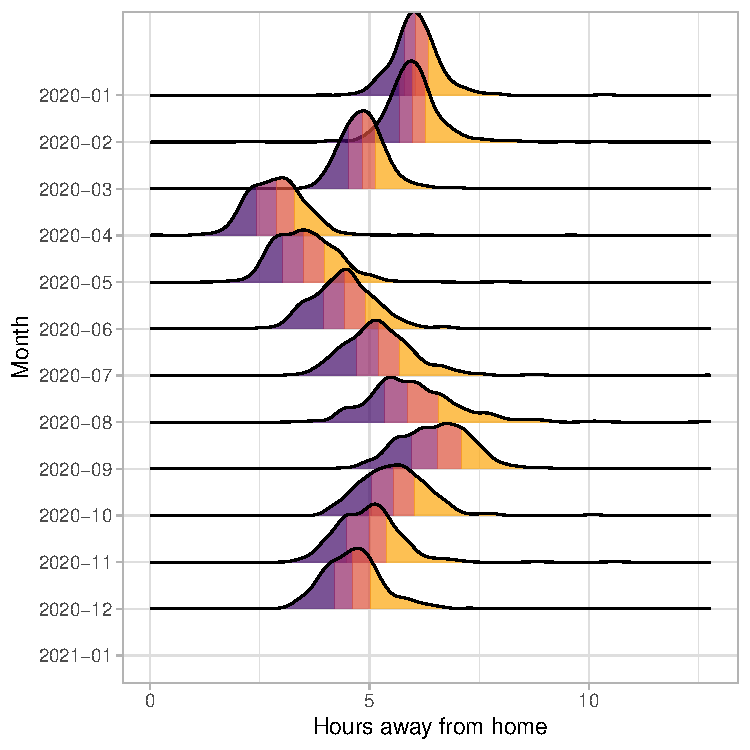
\includegraphics[width=\linewidth]{t-away-hours}
    \caption{Hours away from home}
    \label{fig:W-hours}
  \end{subfigure}
  \begin{subfigure}{0.4\linewidth}
    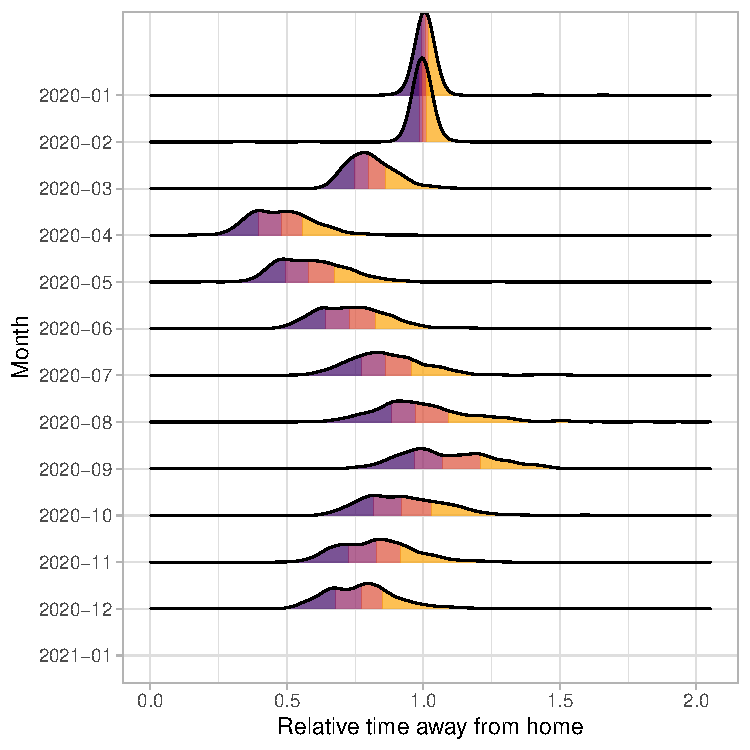
\includegraphics[width=\linewidth]{t-away-relative}
    \caption{Relative time away versus reference period}
    \label{fig:W-relative}
  \end{subfigure}
  \caption{Expected time away from home in hours and versus the reference period (Jan--Feb 2020)}
  \label{fig:W}
  \floatfoot{Distributions show the density of ratio values across all 513 FSAs;
    coloured segments indicate the 4 quantiles of each distributions.}
\end{figure}
\par
Finally, as noted in \S~\ref{ex:data}, Eq.~(\ref{eq:Bgg})\,/\,(\ref{eq:Bgg.app})
can be used to aggregate $B_{nn'}$ to obtain $B_{gg'}$ (repeated here for reference):
\begin{equation}\label{eq:Bgg.app}
  B_{gg'} = \sum_{n \in S_g}\sum_{n' \in S_g'} B^h_{nn'}
\end{equation}
where $S_{g}$ is the set of FSA $n$ corresponding to patch $g$.
% MH: A little bit awkward.
% Do you mean n denotes a set of FSAs?  If so, would recommend putting n in brackets as such:
% "where Sg denotes the set of FSAs (n) corresponding to patch g?"
Figure~\ref{fig:Bggt} illustrates the matrices $B_{gg't}$
for the reference period, and each subsequent month,
% MH: Again a little awkward - would it be fair to say
% "Figure A.4 illustrates monthly matrices ... for the study period,
% with and without inferred mobility within the home decile.
with and without the inferred mobility within the home decile.
% MH: Not showing plots by FSA so would remove this text.
Mobility patterns outlined in Figure~\ref{fig:Bggt} are generally consistent across months,
with the overall proportions of travelling individuals
proportional to the ratio depicted in Figure~\ref{fig:RH0Vt}.
% MH: Would be easier if you could summarize what this ratio is
% rather than forcing individuals to jump back to Figure A.2C to see what this ratio was.
\begin{figure}[ht]
  \centering
  \begin{subfigure}{\linewidth}
    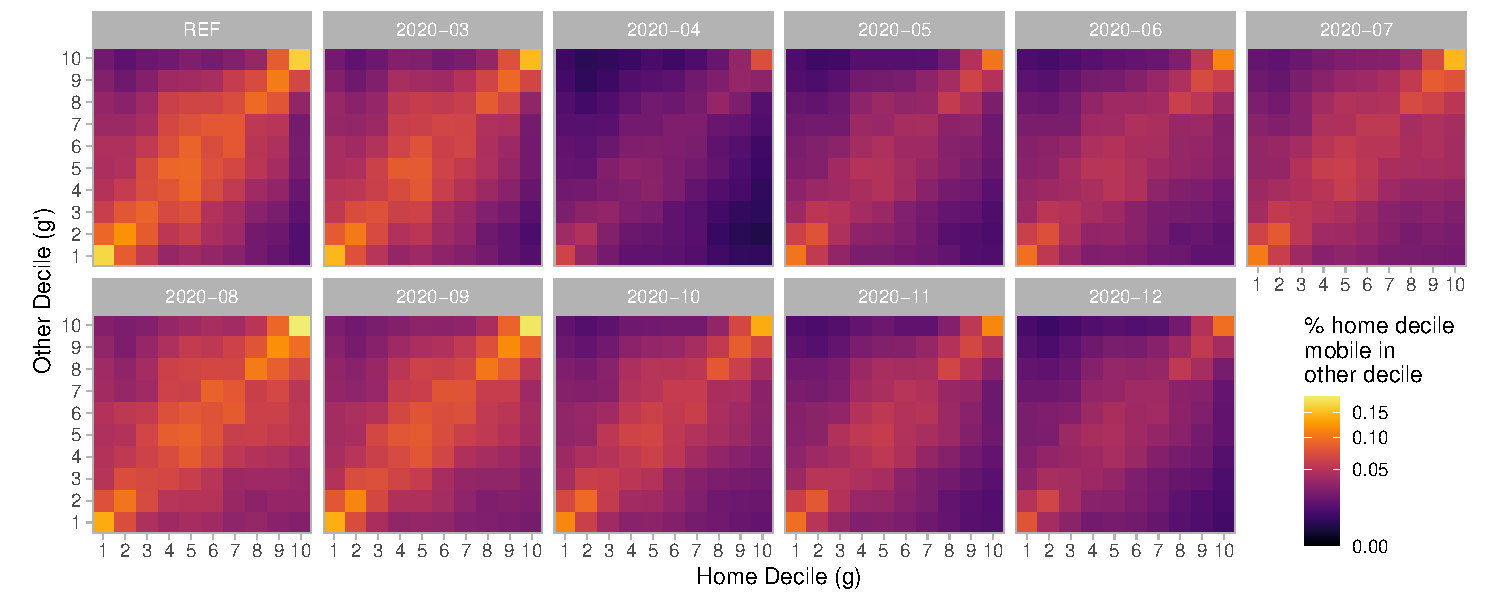
\includegraphics[width=\linewidth]{Bggit}
    \caption{Directly observed mobility: no data for mobility within the residence decile}
    \label{fig:Bggot}
  \end{subfigure}
  \begin{subfigure}{\linewidth}
    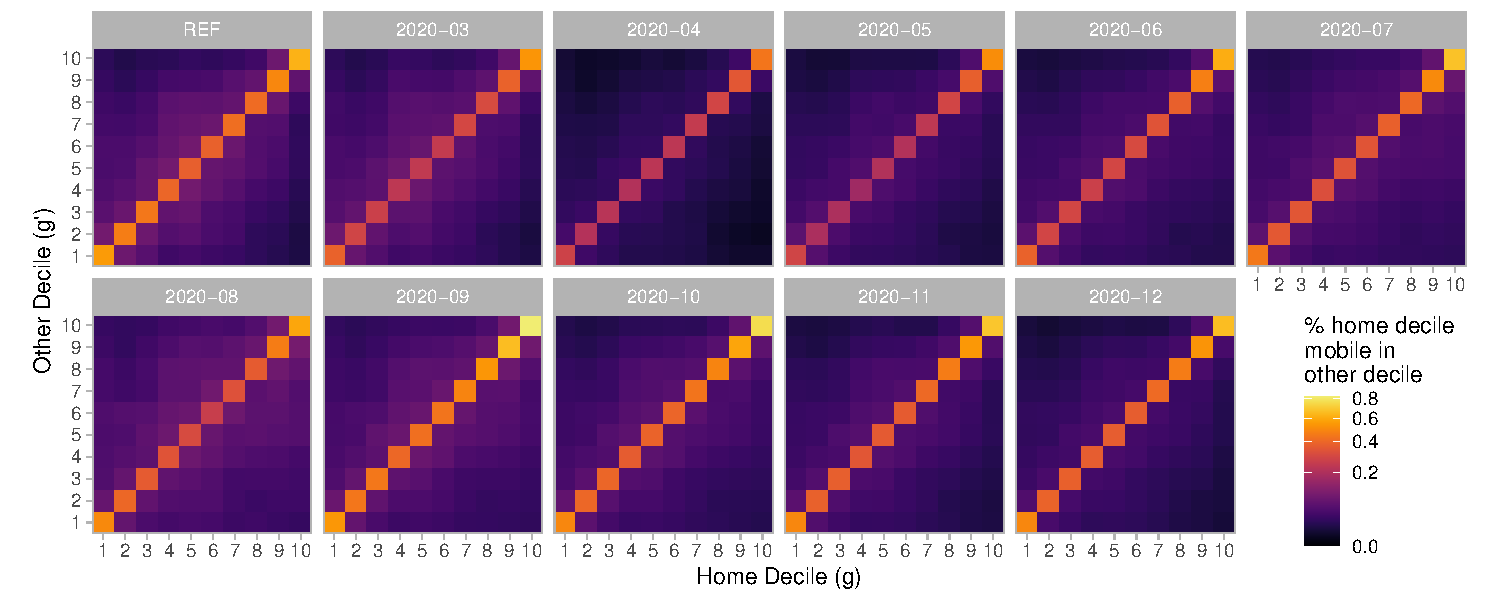
\includegraphics[width=\linewidth]{Bggt}
    \caption{Complete modelled mobility: including inferred mobility within the residence decile}
    \label{fig:Bggdt}
  \end{subfigure}
  \caption{Mobility matrices $B_{gg't}$, representing the expected proportions of individuals
    in patch/decile $g$ who travelled to patch/decile $g'$ each day,
    % MH: Would recommend selecting one or the other rather than stating both patch/decile.
    % Given you have used Decile in your figures, would recommend adding
    % a description of what a decile is so that the figure stands alone from the text.
    stratified by calendar month plus the reference period (Jan--Feb 2020)}
    % MH: Is this additional information neccessary in the title.  Would recommend removing.
    % Instead could add a comment below stating Reference period = January to February 2020
  \label{fig:Bggt}
  \floatfoot{Colour scale is square-root transformed to improve perception of smaller values.}
  % MH: General comment for figures - ensure enough information is present in each figure
  % so that a reader could understand it without reading the manuscript.
  % E.g. provide more information on what a decile is
\end{figure}
\clearpage
% ==================================================================================================
\subsection{Additional Data for Ontario Patches}\label{app.covid}
\begin{figure}[ht]
  \centering
  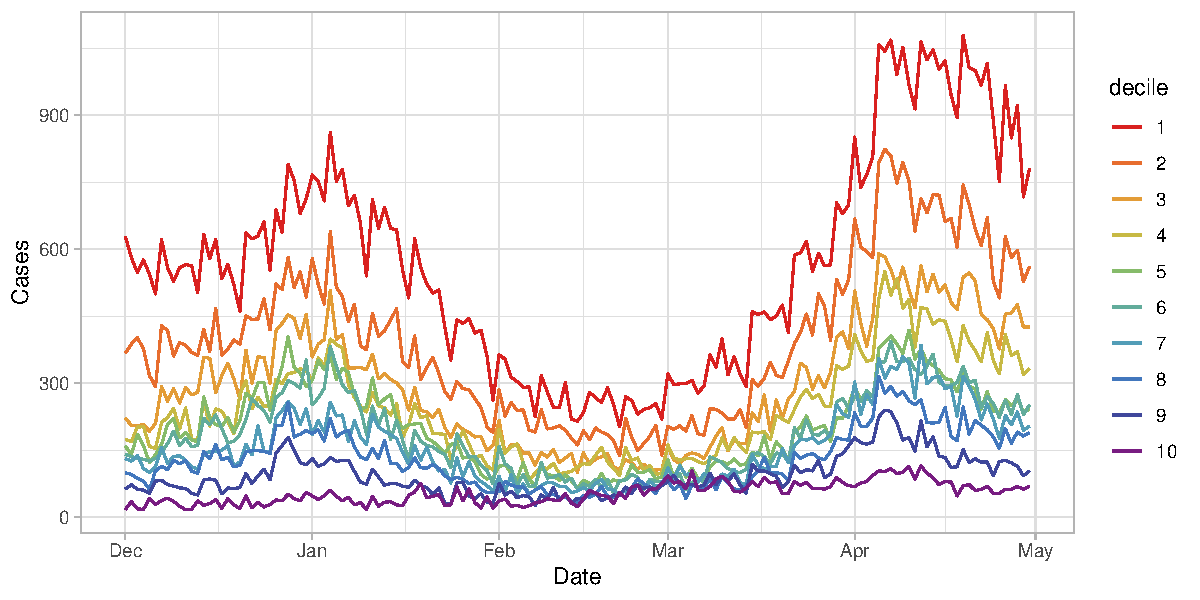
\includegraphics[width=.8\linewidth]{Yg}
  \caption{Time trends in daily \covid cases across the 10 modelled patches in Ontario}
  \label{fig:Yg}
\end{figure}
\begin{figure}[ht]
  \centering
  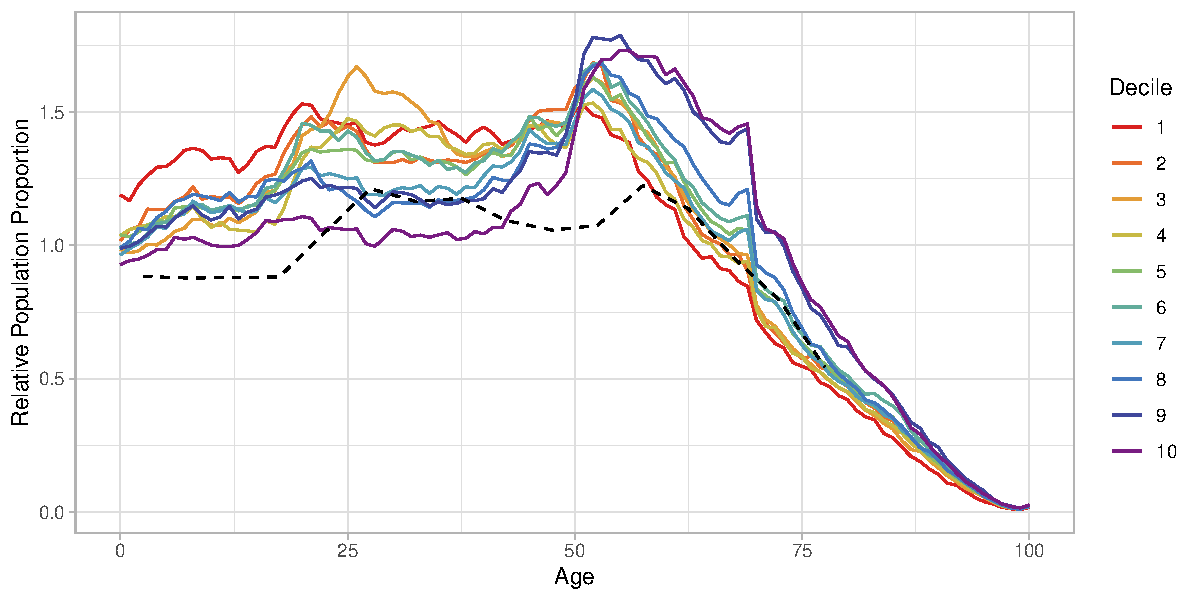
\includegraphics[width=.8\linewidth]{Pga}
  \caption{Population age distributions across the 10 modelled patches in Ontario}
  \label{fig:Pga}
  \floatfoot{Solid coloured lines correspond to the 10 patches defined by
    deciles of cumulative \covid cases between Dec 2020--May 2021 in Ontario.
    Dashed black line corresponds to the Canadian age distribution used by \citet{Prem2017}.}
\end{figure}